\documentclass[tikz,border=3pt]{standalone}
    \usepackage[tt=false,type1=true]{libertine}
    \usepackage[libertine]{newtxmath}
    \usepackage{pgfplots}
    \usepgfplotslibrary{groupplots}
    \pgfplotsset{compat=1.18}
    \definecolor{accent}{HTML}{466E8B}
    \definecolor{graybar}{HTML}{A1A1A1}
    \definecolor{metered}{HTML}{0072B2}
\definecolor{fixed}{HTML}{D55E00}
\definecolor{repzero}{HTML}{0072B2}
\definecolor{repone}{HTML}{D55E00}
\definecolor{reptwo}{HTML}{009E73}
\begin{document}
    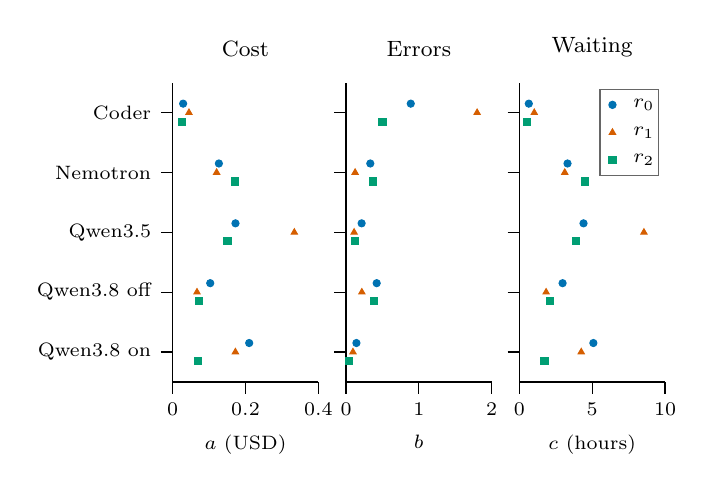
\begin{tikzpicture}
    \begin{groupplot}[
     group style={group size=3 by 1,horizontal sep=10pt},
     width=1.85cm,height=3.8cm,scale only axis,
     ymin=.5,ymax=5.5,ytick={5,4,3,2,1},
     tick label style={font=\fontsize{7.2}{8.2}\selectfont},
     label style={font=\fontsize{7.5}{8.5}\selectfont},
     title style={font=\fontsize{7.8}{8.8}\selectfont},
     tick align=outside,tick style={black,line width=.4pt},
     axis line style={black,line width=.5pt},axis lines*=left,
     scaled ticks=false]
    \nextgroupplot[xmin=0,xmax=0.4,xtick={0,.2,.4},xlabel={$a$ (USD)},title={Cost},yticklabels={Coder,Nemotron,Qwen3.5,Qwen3.8 off,Qwen3.8 on}]
\addplot[only marks,mark=*,mark size=1.3pt,repzero,line width=.35pt] coordinates {(0.028694500,5.150000000)(0.126876442,4.150000000)(0.172438926,3.150000000)(0.103085754,2.150000000)(0.210075746,1.150000000)};
\addplot[only marks,mark=triangle*,mark size=1.3pt,repone,line width=.35pt] coordinates {(0.044711276,5.000000000)(0.120673978,4.000000000)(0.334045041,3.000000000)(0.066762569,2.000000000)(0.172194162,1.000000000)};
\addplot[only marks,mark=square*,mark size=1.3pt,reptwo,line width=.35pt] coordinates {(0.024672116,4.850000000)(0.171422243,3.850000000)(0.150499334,2.850000000)(0.072805326,1.850000000)(0.069025655,0.850000000)};
\nextgroupplot[xmin=0,xmax=2,xtick={0,1,2},xlabel={$b$},title={Errors},yticklabels={}]
\addplot[only marks,mark=*,mark size=1.3pt,repzero,line width=.35pt] coordinates {(0.888888889,5.150000000)(0.333333333,4.150000000)(0.214285714,3.150000000)(0.421052632,2.150000000)(0.142857143,1.150000000)};
\addplot[only marks,mark=triangle*,mark size=1.3pt,repone,line width=.35pt] coordinates {(1.800000000,5.000000000)(0.125000000,4.000000000)(0.111111111,3.000000000)(0.217391304,2.000000000)(0.095238095,1.000000000)};
\addplot[only marks,mark=square*,mark size=1.3pt,reptwo,line width=.35pt] coordinates {(0.500000000,4.850000000)(0.375000000,3.850000000)(0.125000000,2.850000000)(0.384615385,1.850000000)(0.043478261,0.850000000)};
\nextgroupplot[xmin=0,xmax=10,xtick={0,5,10},xlabel={$c$ (hours)},title={Waiting},yticklabels={}]
\addplot[only marks,mark=*,mark size=1.3pt,repzero,line width=.35pt] coordinates {(0.648037210,5.150000000)(3.306793758,4.150000000)(4.404673293,3.150000000)(2.967013377,2.150000000)(5.080503481,1.150000000)};
\addplot[only marks,mark=triangle*,mark size=1.3pt,repone,line width=.35pt] coordinates {(1.022922339,5.000000000)(3.116209026,4.000000000)(8.551730563,3.000000000)(1.836610283,2.000000000)(4.247825485,1.000000000)};
\addplot[only marks,mark=square*,mark size=1.3pt,reptwo,line width=.35pt] coordinates {(0.544635733,4.850000000)(4.515790672,3.850000000)(3.862502242,2.850000000)(2.096995197,1.850000000)(1.729533366,0.850000000)};
\end{groupplot}
    \begin{scope}[shift={([xshift=-19pt,yshift=-8pt]group c3r1.north east)},x=1pt,y=1pt]
     \path[draw=black!60,fill=white,line width=.4pt] (-4.5,5.5) rectangle (16.5,-25.5);
     \draw[only marks,mark=*,mark size=1.3pt,repzero] plot coordinates {(0,0)};
     \node[anchor=west,font=\fontsize{7.2}{8.2}\selectfont] at (4,0) {$r_0$};
     \draw[only marks,mark=triangle*,mark size=1.3pt,repone] plot coordinates {(0,-10)};
     \node[anchor=west,font=\fontsize{7.2}{8.2}\selectfont] at (4,-10) {$r_1$};
     \draw[only marks,mark=square*,mark size=1.3pt,reptwo] plot coordinates {(0,-20)};
     \node[anchor=west,font=\fontsize{7.2}{8.2}\selectfont] at (4,-20) {$r_2$};
    \end{scope}
    \end{tikzpicture}
\end{document}
